\documentclass[a4paper,12pt]{article}
\usepackage{graphicx}  % 用于插入图片
\usepackage{geometry}  % 用于设置页面尺寸
\geometry{margin=1in}  % 设置边距为1英寸
\usepackage{titlesec}  % 用于设置标题样式
\usepackage{setspace}  % 用于设置行距
\usepackage{fancyhdr}  % 用于设置页眉页脚
\usepackage{pdfpages}  % 导入pdfpages宏包
\usepackage{hyperref}
\usepackage{csquotes} 

% 设置行距
\onehalfspacing

% 设置页眉页脚
\pagestyle{fancy}
\fancyhf{}
\rfoot{\thepage}

% 设置标题格式
\titleformat{\section}{\large\bfseries}{\thesection}{1em}{}

% 封面
\begin{document}
\begin{titlepage}
    \centering
    \vspace*{2cm}
    
    \Huge
    \textbf{Individual Report}

    \vspace{1.5cm}

    \Large
    Assignment 2: Individual Report

    \vfill

    \textbf{Mingyuan Ba}\\
    \textbf{SID: 530157791}\\

    \vspace{0.8cm}

    \vfill
\end{titlepage}

% Part A: ER图
\section*{Part A: Extended ER Diagram}
\noindent
This section contains the preliminary extended ER diagram. Here are links to \hyperlink{PartB}{Part B} and \hyperlink{PartC}{Part C}

% 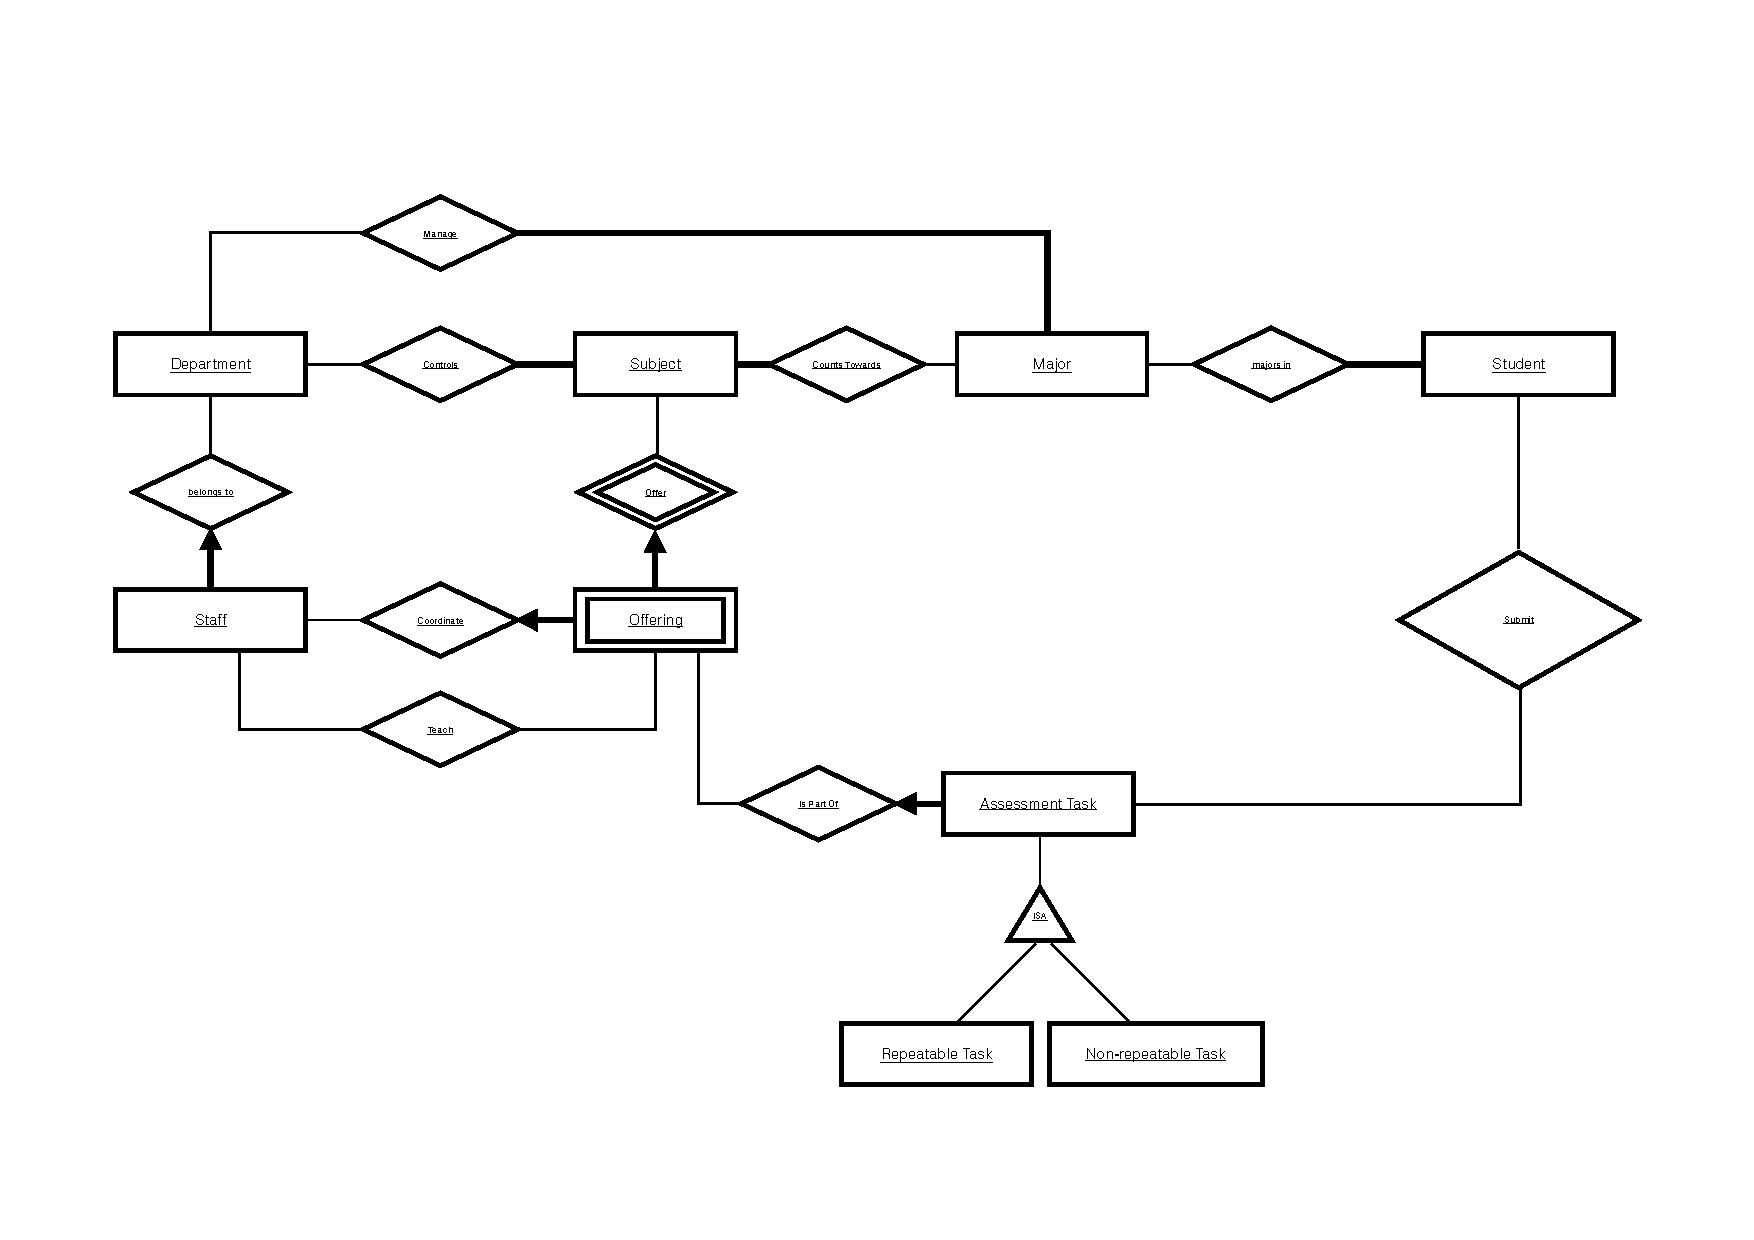
\includepdf[pages={1-5}]{Graphs/ER-diagram_1.pdf}

\newpage

% Part B: 检查过程描述
\section*{Part B: Diagram Validation and Checking Process}
\hypertarget{PartB}{}
\noindent
In this section, I describe how I checked the ER diagram for validity and correctness based on the system's textual description. The following checks were performed:

\begin{itemize}
  \item \texttt{The system needs to keep a scan of every submission made by a student for an assessment task.A submission is handed in at a date and time which must be recorded, and it may have been awarded a mark by a staff member.}

  This sentence indicates a many to many relationship from student to assessment task with attributes \texttt{date}, \texttt{time} and \texttt{mark}. According to Ed post \texttt{\#497}, we should also record which \texttt{staff} marked this submission. However, this information cannot be represented in the current ER diagram.

  \item \texttt{The system needs to keep information for each student, including their studentkey (an identifier such as JS2X57), surname, given name, year-of-entry, major(s), official email, and address}

  For this description, we can model \texttt{Student} as an entity set, with attributes including \texttt{studentkey,surname, given name, year-of-entry, major(s), official email,} and \texttt{address}.

  In the ER diagram, I have introduced a \texttt{Student} entity with attributes such as \texttt{studentkey (PK)} and the other attributes mentioned above.

  \item \texttt{Staff members are identified by staffId, and have surname, given name, title, department, official email, and contact phone number. }

  Based on the description, we need to introduce \texttt{Staff} as an entity set, with attributes including \texttt{surname, given name, title, department, official email}, and \texttt{contact phone number}.

  The ER diagram does show the \texttt{Staff} entity and its attributes.

  \item \texttt{Each assessment task occurs for an offering of a subject [for example, the offering of the subject Traditional Philosophy in sem1 of 2024], and the assessment task has a name (eg “Assignment 1”), a weight towards the grade in the offering, a kind (such as Essay, Quiz, ProblemSet, FinalExam), an instruction document, and a latest-date-for-submission.}

  These sentences describes an entity set \texttt{Assessment Task} with the attributes: \texttt{Name, Weight, Kind, LatestDate}, and \texttt{Instruction Document}. Since each \texttt{Assessment Task} must belong to a specific \texttt{Offering}, there is a many-to-one relationship from \texttt{Assessment Task} to \texttt{Offering}. Due to the possibility of different assessment tasks having the same name, I have added a new attribute, \texttt{AssessmentId}, to uniquely identify them. The diagram indeed represents entity set and relationship mentioned above.

  In addition, \texttt{Offering} as an Entity Set needs to be identified through \texttt{Subject, year, and semester} (according to Ed post \texttt{\#399}). This indicates that \texttt{Offering} is a Weak Entity Set, where both \texttt{year} and \texttt{semester} are discriminators, and this is clearly represented in the diagram.


  \item \texttt{Some assessment tasks are non-repeatable; this means that a student may not submit for this more than once, and in that case, there is a mechanism for the student to request an exemption for illness (the system needs to track the text of the request, the date it was made, and whether or not this was approved). For an assessment which does allow multiple submissions, we need to keep information on a policy which decides how to calculate the overall score the student gets (for example, it may be that only the latest submission is marked, or that each submission is marked and the highest mark is used, or maybe the latest submission is marked but a penalty is subtracted based on the number of submissions made). }

  This description explains that Assessment Tasks can be divided into two categories: Repeatable and Non-Repeatable, each with different attributes to be recorded. Our diagram indeed represents this by creating an \texttt{ISA} structure, where the common attributes are stored in the \texttt{Assessment Task} entity, and the specific attributes are stored separately in \texttt{Repeatable Task} and \texttt{Non-Repeatable Task}.

  \item \texttt{For a subject, we need to know its name, the credit-hours it carries, the major(s) it counts towards [if any], and whether or not students are allowed to take it more than once.}

  This statement clearly indicates that \texttt{Subject} should be represented as an entity set, and its attributes should include the \texttt{name, credit hours, and whether it allows retaking}. Additionally, each subject may be associated with zero or more majors, highlighting a many-to-many relationship between \texttt{Subject} and \texttt{Major}. However, there are two errors in the diagram: First, the relationship between \texttt{Subject} and \texttt{Major} is incorrectly depicted as requiring all subjects to participate in this relationship, when in reality, a subject may not belong to any major. Second, the \texttt{Subject} entity should not have multi-valued attributes, as this aspect is already captured by the relationship.

  \item \texttt{The same subject may be taught over several offerings and the assessment tasks will be different between these offerings (though they may share a name!)}

  This statement clarifies that the relationship from \texttt{Subject} to \texttt{Offering} should be one-to-many, with all Offerings participating in this relationship. Additionally, the relationship between \texttt{Assessment Task} and \texttt{Offering} should be many-to-one, with all Assessment Tasks required to participate. These relationships are clearly represented in the diagram using bold arrows. Considering that Assessment Tasks may have the same name, the diagram introduce an attribute \texttt{AssessmentID} to distinguish between them.

  \item \texttt{Each offering is taught by a staff member as coordinator, and possibly there are other staff as teachers as well. }

  In this description, we can identify two distinct relationships between Staff and Offering:
  \begin{enumerate}
    \item A many-to-one relationship from \texttt{Offering} to \texttt{Staff}, where every Offering is associated with exactly one coordinator. This means that each \texttt{Offering} has exactly one coordinator.

    \item A many-to-many relationship, indicating that an \texttt{Offering} can be taught by multiple Staff members, and a single Staff member can teach multiple Offerings.
  \end{enumerate}

  The current diagram accurately represents both of these relationships.


  \item \texttt{The staff are each members of a department, and every subject is under control of some department.}

  The description reflects two relationships:
    \begin{enumerate}
        \item Staff should belong to a department, but due to the unclear phrasing, the specific type of relationship in the diagram is still open for discussion.

        \item Every subject should be controlled by a department, but the description does not specify whether it can be controlled by multiple departments.
    \end{enumerate}
  The relationships depicted in the current diagram may not cover all potential cases, and further discussion is required.

  \item \texttt{A department may be responsible for a major (and indeed, some majors may be shared between departments, eg “Greek History” major is shared between Classics department and History department).}

  A many-to-many relationship from department to major is reflected in this statement. However, since it does not clearly specify whether all majors must be managed by a department, the specific details of the relationship remain unclear. The diagram currently assumes that all majors must be part of the relationship.




\end{itemize}

\newpage

% Part C: 小组工作过程描述
\section*{Part C: Group Process Description}
\hypertarget{PartC}{}
\noindent
The group followed a collaborative process to produce the conceptual model and the final report. Below is a breakdown of the tasks and contributions:

\begin{itemize}
    \item \textbf{Task Assignment:} Each group member was assigned specific tasks. I was responsible for validating the ER diagram, while other members worked on the final model and report writing.
    
    \item \textbf{Meetings and Discussions:} We held regular meetings to discuss progress and ensure that everyone was on track. Disagreements, such as the interpretation of certain business rules, were resolved through discussion and consensus.

    \item \textbf{Strengths of the Process:} The process was efficient in distributing the workload, and each member was able to focus on their assigned task, ensuring that the final report was completed on time.

    \item \textbf{Limitations and Suggestions for Improvement:} One limitation of our process was the lack of early reviews of the diagram, which could have identified issues sooner. In future assignments, we suggest implementing earlier peer reviews to catch potential problems earlier in the design phase.
\end{itemize}

\end{document}

